% Apéndice Materiales Magnéticos

\chapter{Materiales Magnéticos.} % Main appendix title

\label{AppendixMaterialesMagneticos} % For referencing this appendix elsewhere, use \ref{AppendixA}

%\section{Materiales magnéticos.}

Los materiales magnéticos se pueden clasificar en cinco grandes grupos de acuerdo a sus propiedades y su comportamiento frente a campos magnéticos externos. Estos comportamientos resultan del acoplamiento de magnitudes propias de los átomos (momento angular total, espín y momento magnético intrínseco) con su ordenamiento en estructuras moleculares y cristalinas. Como el ordenamiento y las estructuras dependen fuertemente de la temperatura, hay temperaturas críticas en las que ocurren transiciones entre los grupos. 

%\subsection{Materiales con magnetismo intrínseco.}
\section{Materiales con magnetismo intrínseco.}

El magnetismo intrínseco se manifiesta cuando el campo de cada átomo individual no afecta a los átomos vecinos. No hay manifestación de interacciones cooperativas:

\begin{itemize}

	\item \textbf{Materiales diamagnéticos:}
el diamagnetismo es una propiedad fundamental de toda la materia. Se debe al comportamiento no cooperativo de los electrones cuando se exponen a un campo magnético exterior. El resultado es la generación de un débil campo opuesto al campo externo. Se observa muy claramente en los sistemas atómicos, iónicos y moleculares que contienen todos sus electrones apareados o que tengan orbitales completamente llenos. Como el momento inducido sólo depende del tamaño y de la forma de los orbitales en las capas completas y esto no depende de la temperatura, el diamagnetismo dependerá muy poco de la temperatura en condiciones normales. A temperaturas muy bajas en los metales el diamagnetismo presenta fuertes variaciones con la temperatura y violentas oscilaciones frente variaciones pequeñas del campo exterior. Esto se conoce como efecto De Hass-van Alphen\footnote{\url{https://en.wikipedia.org/wiki/De\_Haas-van\_Alphen\_effect}}. Ya que el diamagnetismo es función de la distribución electrónica es mas importante en los compuestos que contengan átomos con mayor numero de electrones.
En la práctica la mayoría de los materiales compuestos pertenecen a este grupo.

	\item \textbf{Materiales paramagnéticos:} 
en esta clase de materiales algunos de los átomos o iones cristalinos tienen un momento magnético neto debido a electrones no pareados en orbitales parcialmente llenos. Se manifiesta por la aparición de un fuerte campo magnético debido a la alineación individual de los momentos magnéticos de los átomos o moléculas en forma paralela a la del campo magnético externo. Debido a la agitación térmica el paramagnetismo desaparece  cuando se retira el campo magnético externo; esto se debe a que la agitación térmica distribuye aleatoriamente la dirección de los dipolos magnéticos lo que lo hace altamente dependiente de la temperatura y un aumento de ella disminuye el efecto paramagnético. Son paramagnéticos todos los átomos y moléculas que poseen un número impar de electrones, pues presentan un momento magnético neto i.e. el spín total del sistema no debe ser nulo, por ejemplo átomos libres de Na y óxido nítrico gaseoso (NO). También son paramagnéticos todos los átomos y iones libres con una capa interna incompleta, por ejemplo elementos de transición como el Mn y el Gd y los elementos con una capa exterior incompleta: C, Ni, O, Fl, Al, Cu, Fe, Co, Ni, etcétera. Cuando los átomos dejan de estar libres las uniones moleculares y cristalinas hacen que la mayoría de los materiales compensen sus espínes y se vuelvan diamagnéticos. 

\end{itemize}


%\subsection{Materiales con magnetismo extrínseco.}
\section{Materiales con magnetismo extrínseco.}

El magnetismo extrínseco se manifiesta cuando los campos generados en cada átomo individual actuan colectivamente generándose ordenaciones macroscópicas capaces de generar un campo magnético propio en el material

\begin{itemize}

	\item \textbf{Materiales ferromagnéticos:} 
son materiales donde los campos de los átomos exhiben interacciones cooperativas muy fuertes constituyendo regiones de dominios magnéticos más allá de los dominios cristalinos, esto produce una intensa magnetización permanente aún en ausencia de campos exteriores. A este grupo pertenecen muchos materiales basados en hierro, níquel, cobalto, gadolinio, disprosio, sus aleaciones y algunos de sus óxidos, aunque notablemente no está entre ellos la magnetita ($Fe^{2+}Fe^{3+}_{2}O_{4}$). EL ferromagnetismo no es exclusividad sólo de los elementos citados, hay aleaciones que no contienen a ninguno de ellos y son ferromagnéticas por ejemplo las aleaciones Heusler $Cu_{2}MnAl$ y por el contrario también tenemos aleaciones de hierro que no son ferromagnéticas como los aceros inoxidables austeníticos; incluso bajo ciertas condiciones de presión y temperatura el hierro no es ferromagnético. El $Fe-\alpha$ llamado ferrita es una estructura cristalina del tipo cúbica centrada en el cuerpo (ccb) que presenta las mejores propiedades magnéticas del Fe puro; se suele alear con cobalto y bario para hacer imanes permanentes. Existen aleaciones que presentan un ferromagnetismo muy intenso y se conocen por sus nombres comerciales: Permalloy, Hipernik, Monimax, Permendur, Superpermalloy, Hiperco, Ferroxcube III, etcétera.

	\item \textbf{Materiales antiferromagnéticos:}
son materiales compuestos donde cada componente presenta momentos magnéticos opuestos casi iguales, resultando en un momento neto muy pequeño en ausencia de campos exteriores. Estos materiales se pueden pensar como dos subredes cristalinas dispuestas de forma tal, que cada una por separado podría presentar un momento magnético neto como los ferromagneticos, pero juntas cada una es afectada por la presencia de la otra y se ordenan como un material ferromagnético, pero con los momentos netos de cada subred en direcciones opuestas. Este ordenamiento antiparalelo puede aparecer en presencia de un campo magnético exterior, cancelándose si tienen el mismo valor absoluto o reduciéndolo si son distintos. Si el campo magnético externo es lo bastante intenso algunos de los momentos magnéticos opuestos se alinean paralelamente con él, aun a costa de alinearse en paralelo a sus vecinos superando la interacción antiferromagnética y volviéndose paramagnético. Ejemplo: la hematita ($\alpha FE_{2}O_{3}$)

	\item \textbf{Materiales ferrimagnéticos:}
el ferrimagnetismo es similar al antiferromagnetismo pero las subredes involucradas tienen momentos magnéticos opuestos de muy diferente magnitud. Esto produce la aparición campo magnéticos inducidos grandes e inclusive su aparición en forma espontánea similarmente a los ferromagnéticos. Los ordenamientos son mas complejos que los antiferromagnéticos y uno de ello da nombre al grupo. La magnetita es un sólido ferrimagnetico ($Fe^{2+}Fe^{3+}_{2}O_{4}$) aunque por siglos fue el ejemplo de ferromagnetismo. El $Mn_{12}$ es una molécula con interacciones antiferromagnéticas que presenta un momento magnético grande del estado fundamental. Existen sistemas antiferromagnéticos incluidos en este grupo que presentan magnetización permanente pero los momentos no son totalmente antiparalelos sino que presentan pequeñas desviaciones angulares del alineamiento de los momentos magnéticos resultando en dos direcciones netas opuestas para cada subred. Los materiales ferrimagnéticos se conocen con el nombre de ferritas.

\end{itemize}

\section{Características comunes a todos los grupos.}

A altas temperaturas los materiales tenderán a ser diamagnéticos o paramagnéticos.
En la Figura \ref{fig:suceptibilidades} podemos ver distintas transiciones entre los grupos y las temperaturas críticas a las que ocurren en función de la susceptibilidad \footnote{\url{https://en.wikipedia.org/wiki/Magnetic\_susceptibility}} \raisebox{\depth}{\scalebox{1.25}{$\chi$}}. 


\begin{figure}[h]
	\centering
	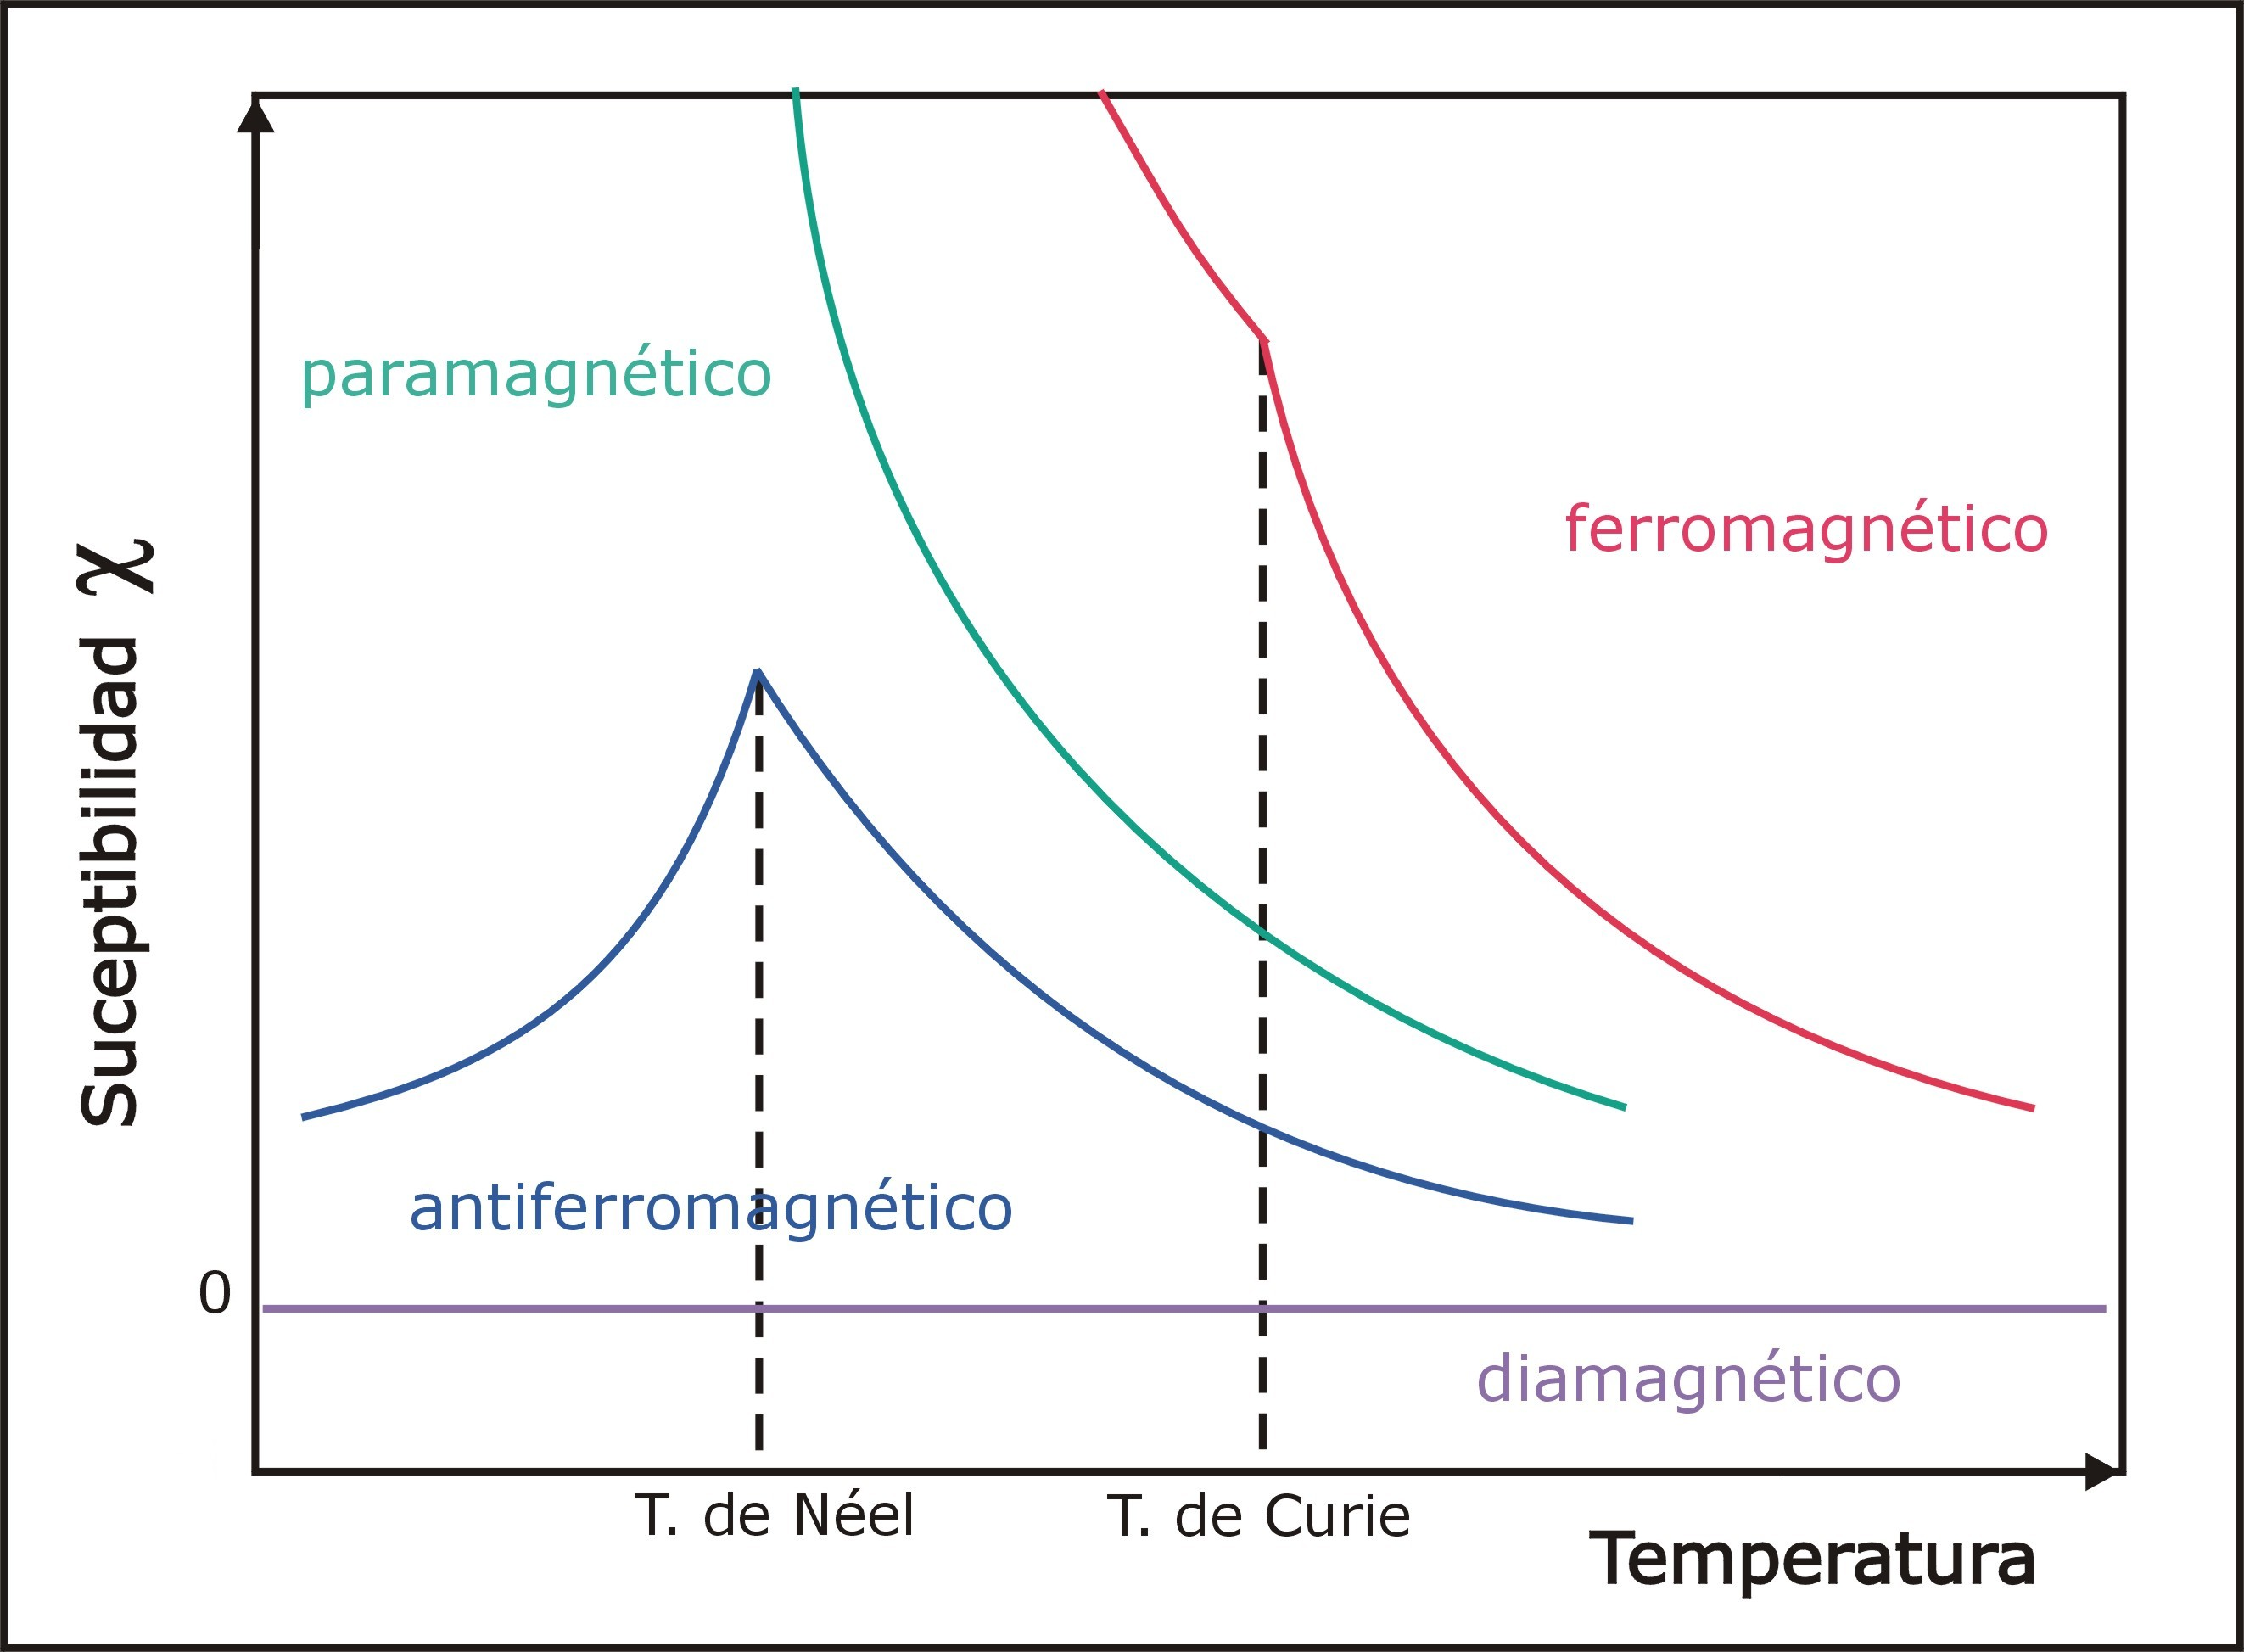
\includegraphics[width=0.75\textwidth]{./Figures/suceptibilidades}
	\caption{Suceptibilidad magnética y temperaturas de transición entre los distintos grupos.}
	\label{fig:suceptibilidades}
\end{figure}.



En el vacío \raisebox{\depth}{\scalebox{1.25}{$\chi$}} vale cero y en ese caso diríamos que el material en amagnético, cuando \raisebox{\depth}{\scalebox{1.25}{$\chi$}}$<0$ tendremos los diamagnéticos y cuando \raisebox{\depth}{\scalebox{1.25}{$\chi$}}$>0$ los restantes. Aplicando la definición de permeabilidad magnética $\mu = \mu_{0}(1+$\raisebox{\depth}{\scalebox{1.25}{$\chi$}}$)$ definiendo el $\mu$ relativo como: $\mu_{r}=(1+$\raisebox{\depth}{\scalebox{1.25}{$\chi$}}$)$ tendremos que para los materiales amagnéticos será $\mu_{r}=1$, para los diamagnéticos $\mu_{r}<1$ y para el resto $\mu_{r}>1$ tal como podemos ver en la figura \ref{fig:Permeability}



\begin{figure}[h]
	\centering
	$\mu_{f}$ ferromagnéticos, $\mu_{p}$ paramagnéticos, $\mu_{0}$ vacío, $\mu_{d}$ diamagnéticos.
	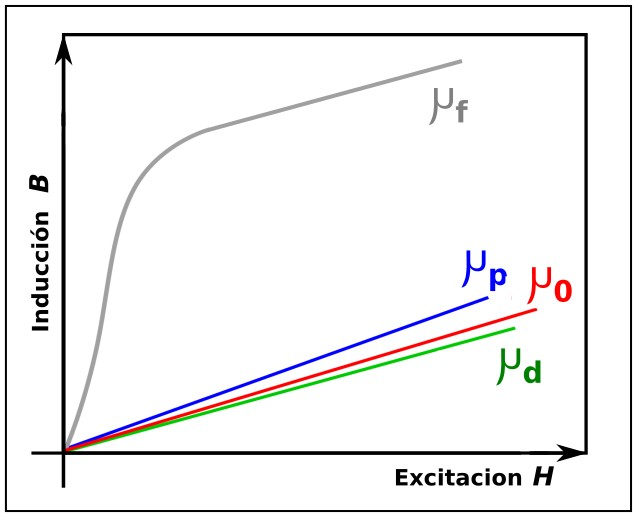
\includegraphics[width=0.75\textwidth]{./Figures/permeabilidad2.jpg}
	\caption{Permeabilidad magnética $\mu$ inducción $B$ vs. excitación $H$.}
	\label{fig:Permeability}
\end{figure}.


